\documentclass{standalone}
\usepackage{tikz}
\usepackage{ctex,siunitx}
\setCJKmainfont{Noto Serif CJK SC}
\usepackage{tkz-euclide}
\usepackage{amsmath}
\usepackage{wasysym}
\usetikzlibrary{patterns, calc}
\usetikzlibrary {decorations.pathmorphing, decorations.pathreplacing, decorations.shapes,}
\begin{document}
\small
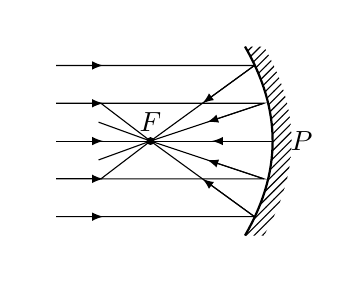
\begin{tikzpicture}[>=latex,scale=1.2]
  \useasboundingbox(-0.3,1.2)rectangle(2.9,-1.2);
  \fill [pattern=north east lines] (2,-1)--(2.2,-1) to [bend left=-30] (2.2,1) --(2,1) to [bend left=30](2,-1);
  \draw [thick](2,1) to [bend left=30] (2,-1);
  \foreach \x in {-.8,-.4,0,...,.8}
  {
    \draw[->] (0,\x)--(0.5,\x);
  }    
  \draw  (0,-.8)--(2.1,-.8)--(1,0)--(.95/2,.4);
  \draw  (0,.8)--(2.1,.8)--(1,0)--(.95/2,-.4);
  \draw  (0,-.4)--(2.2,-.4)--(1,0)--(.9/2,.2);
  \draw  (0,.4)--(2.2,.4)--(1,0)--(.9/2,-.2);
  \draw  (0,0)--(2.3,0);
  \draw[->](2.1,-.8)--(3.1/2,-.4);  
  \draw[->](2.1,.8)--(3.1/2,.4);
  \draw[->](2.2,-.4)--(3.2/2,-.2);   
  \draw[->](2.2,.4)--(3.2/2,.2);
  \draw[->] (2.3,0)--(3.3/2,0);
  \node at (1,0)[above]{$F$};      
  \node at (2.6,0){$P$};   
  \draw (1,0)[ fill=black] circle (1pt);
\end{tikzpicture}
\end{document}